%%%%%%%%%%%%%%%%%%%%%%%%%%%%%%%%%%%%%%%%%
% Beamer Presentation
% LaTeX Template
% Version 1.0 (10/11/12)
%
% This template has been downloaded from:
% http://www.LaTeXTemplates.com
%
% License:
% CC BY-NC-SA 3.0 (http://creativecommons.org/licenses/by-nc-sa/3.0/)
%
%%%%%%%%%%%%%%%%%%%%%%%%%%%%%%%%%%%%%%%%%

%----------------------------------------------------------------------------------------
%	PACKAGES AND THEMES
%----------------------------------------------------------------------------------------

\documentclass{beamer}

\mode<presentation> {

% The Beamer class comes with a number of default slide themes
% which change the colors and layouts of slides. Below this is a list
% of all the themes, uncomment each in turn to see what they look like.

%\usetheme{default}
%\usetheme{AnnArbor}
%\usetheme{Antibes}
%\usetheme{Bergen}
%\usetheme{Berkeley}
\usetheme{Berlin}
%\usetheme{Boadilla}
%\usetheme{CambridgeUS}
%\usetheme{Copenhagen}
%\usetheme{Darmstadt}
%\usetheme{Dresden}
%\usetheme{Frankfurt}
%\usetheme{Goettingen}
%\usetheme{Hannover}
%\usetheme{Ilmenau}
%\usetheme{JuanLesPins}
%\usetheme{Luebeck}
%\usetheme{Madrid}
%\usetheme{Malmoe}
%\usetheme{Marburg}
%\usetheme{Montpellier}
%\usetheme{PaloAlto}
%\usetheme{Pittsburgh}
%\usetheme{Rochester}
%\usetheme{Singapore}
%\usetheme{Szeged}
%\usetheme{Warsaw}

% As well as themes, the Beamer class has a number of color themes
% for any slide theme. Uncomment each of these in turn to see how it
% changes the colors of your current slide theme.

%\usecolortheme{albatross}
%\usecolortheme{beaver}
%\usecolortheme{beetle}
%\usecolortheme{crane}
\usecolortheme{dolphin}
%\usecolortheme{dove}
%\usecolortheme{fly}
%\usecolortheme{lily}
%\usecolortheme{orchid}
%\usecolortheme{rose}
%\usecolortheme{seagull}
%\usecolortheme{seahorse}
%\usecolortheme{whale}
%\usecolortheme{wolverine}

%\setbeamertemplate{footline} % To remove the footer line in all slides uncomment this line
%\setbeamertemplate{footline}[page number] % To replace the footer line in all slides with a simple slide count uncomment this line

%\setbeamertemplate{navigation symbols}{} % To remove the navigation symbols from the bottom of all slides uncomment this line
}

\usepackage{graphicx} % Allows including images
\usepackage{booktabs} % Allows the use of \toprule, \midrule and \bottomrule in tables
\usepackage{hyperref}
\usepackage[utf8]{inputenc}
\usepackage{rotating}
\usepackage[export]{adjustbox}

%----------------------------------------------------------------------------------------
%	TITLE PAGE
%----------------------------------------------------------------------------------------

\title[Lehrvortrag. Geoinformation in der Landschaftsplanung. 2018]{Geoinformation in der Landschaftsplanung:\\Techniken, Methoden und Anwendung am Beispiel eines Schutzgutes\\
\medskip \tiny{Lehrvortrag, Hochschule Geisenheim University}} % The short title appears at the bottom of every slide, the full title is only on the title page

\author[Avit Bhowmik]{\textbf{Dr. Avit K. Bhowmik} \\
The Royal Swedish Academy of Sciences} % Your name
\institute[The Royal Swedish Academy of Sciences] % Your institution as it will appear on the bottom of every slide, may be shorthand to save space
{
\textit{avit.bhowmik@futureearth.org}% Your email address
}
\date[\today]{\today \\[0.2cm]

\includegraphics[width=0.25\textwidth]{Figures/KVA_logo.png}

\includegraphics[width=0.26\textwidth]{Figures/FE_logo.png}} % Date, can be changed to a custom date

\begin{document}

\begin{frame}
\titlepage % Print the title page as the first slide
\end{frame}

%------------------------------------------------

\begin{frame}
  \frametitle{Kontext des Lehrvotrages}
\begin{itemize}
\item Studiengang: B.Sc. Landschaftsarchitektur, M.Sc. Umweltmanagement und Stadtplanung in Ballungsräumen
\item Potenzieller Kurs: Fundamentale und angewandte Geoinformatik
\item \alert{Potenzielle Kursinhalte}:
\begin{itemize}
\item Einführung: Was ist GIS?
\item Was ist der Nutzen von GIS in der Landschaftsplanung? 
\item Techniken und Methoden
\end{itemize}
\end{itemize}
\end{frame}
%------------------------------------------------

\begin{frame}
  \frametitle{Erwartungen und Lernziele}
\begin{itemize}
\item \alert{Eure Erwartungen:} Umfrage vor Kursbeginn, z.B. Surveymonkey
\item \alert{Meine Erwartungen:}
\begin{itemize}
\item Rückfragen und kritisches Denken
\item “Problembasiertes Lernen”
\end{itemize}
\item \alert{Lernziele:}
\begin{itemize}
\item Verständnis von Grundlagen und Eigenschaften raumzeitlicher Informationsysteme und -wissenschaft
\item Transfer des Gelernten auf die Landschaftsplanung
\end{itemize}
\item Inhalt der Vorlesung kann online under dem folgenden Link abgerufen werden: \alert{https://github.com/AvitBhowmik/testGU}
\end{itemize}
\end{frame}
%------------------------------------------------

\begin{frame}
\frametitle{Was wissen wir bereits?}
\centering
\Huge \alert{Was ist GIS?}\\
\vspace{1cm}

\includegraphics[width=0.4\textwidth]{Figures/Questions.png}
\end{frame}

%------------------------------------------------

\begin{frame}
\centering
\Huge \alert{\textbf{GIS}}\\
\pause
\Large \textbf{? Information ?}
\pause
\medskip
\normalsize
\begin{columns}[t]
\column{.6\textwidth}
\begin{itemize}
\item \alert{\textbf{Geographisch}}\\
Parent and Church, 1987. Conf. GIS
\item \alert {\textbf {Räumlich (Geospatial)}}\\
Anselin, 1989. What is special about spatial data?
\item \alert{\textbf{Raumzeitlich}}\\
Burrough and Frank, 1995. Int J GIS
\end{itemize}
\hspace{2cm}
\pause
\column{.5\textwidth}
\begin{itemize}
\item \alert{\textbf{System}}\\
CCS, 1975
\item \alert{\textbf{Wissenschaft}}\\
Goodchild, 1992. Int J GIS
\end{itemize}
\end{columns}
\end{frame}

%------------------------------------------------

\begin{frame}
\frametitle{Setzt die GIS Brille auf}
\centering

\includegraphics[width=0.5\textwidth]{Figures/GIglass.png}\\
\pause
\textbf{Landschaftsplanung in Hessen:}\footnotesize
\begin{itemize}
\item Berücksichtigung des Naturschutzes und der Landschaftspflege
\item Zweistufige Landschaftsplanung: örtlich und überörtliche
\end{itemize}
\end{frame}

%------------------------------------------------

\begin{frame}
\frametitle{GIS in der Landschaftsplanung}
\centering
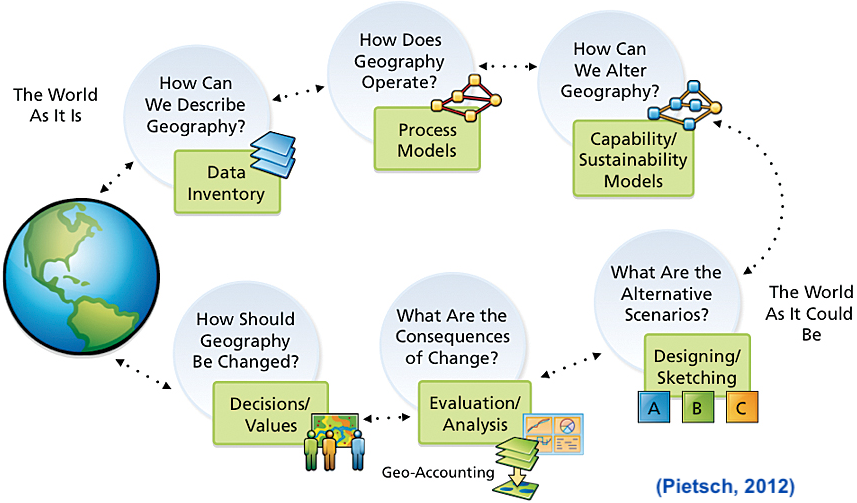
\includegraphics[width=1.07\textwidth]{Figures/gis_app.png}
\end{frame}

%------------------------------------------------

\begin{frame}
\frametitle{}
\centering
\Huge \alert{Techniken und Methoden}\\[0.5cm]
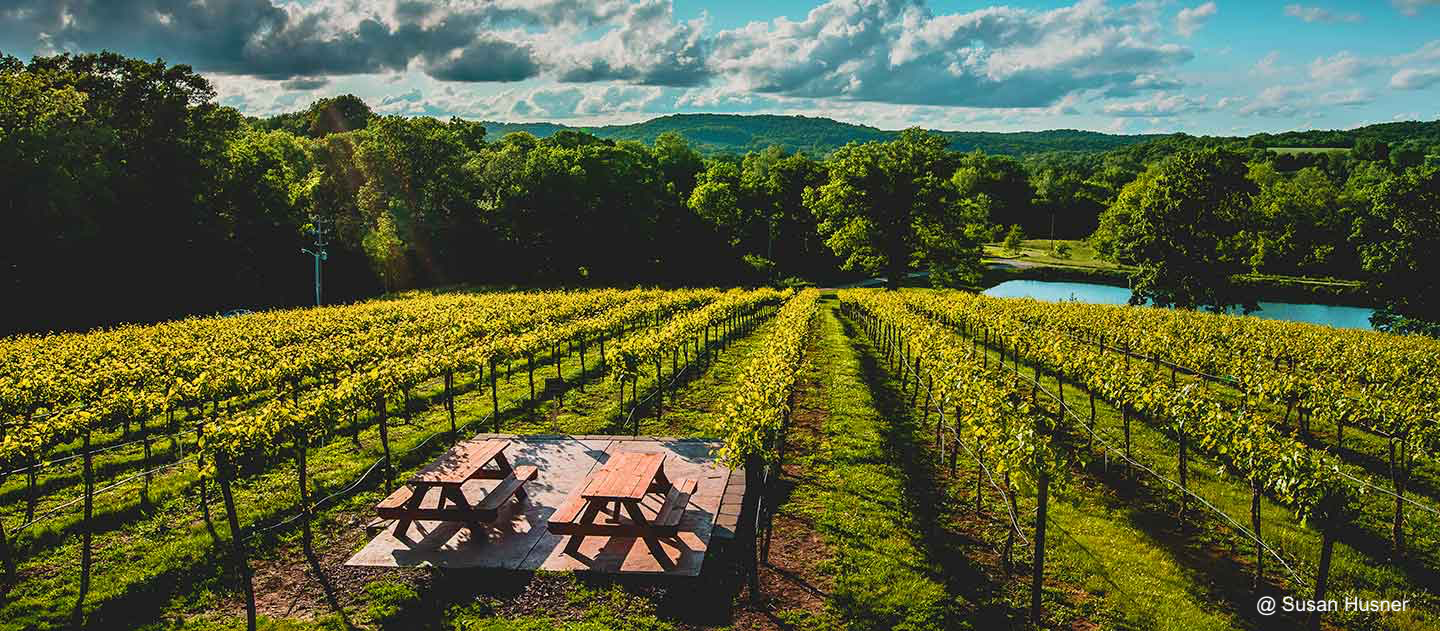
\includegraphics[width=\textwidth]{Figures/wine.png}
\end{frame}

%------------------------------------------------

\begin{frame}
\frametitle{Raumzeitliche (Geo-) Statistik}
\onslide<1->
\begin{columns}
\column{.6\textwidth}
\alert{Erstes Gesetz der Geographie}\\[0.5cm]
``Everything is related to everything else, but near things are more related to each other''\\[0.5cm]
\onslide<2->
\textbf{Räumliche Autokorrelation}\\
\onslide<1->
\hspace{2cm}
\column{.4\textwidth}
\raggedleft
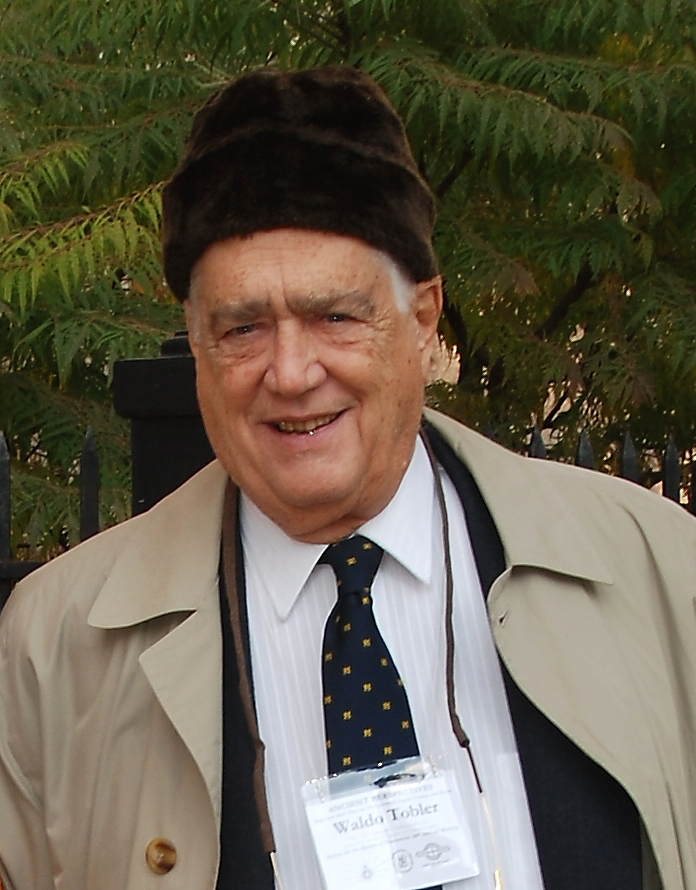
\includegraphics[width=0.85\textwidth]{Figures/Tobler_2007.png}\\
\tiny Foto: Professor Dr. Waldo Tobler, 2007
\end{columns}
\end{frame}

%-----------------------------------------------

\begin{frame}
\frametitle{Raumzeitliche (Geo-) Statistik}
Raumzeitliche Interpolation\\
\centering
$\vcenter{\hbox{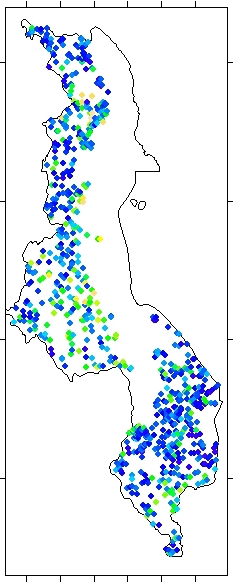
\includegraphics[width=0.25\textwidth]{Figures/Mwipt.png}}}$
\hspace{1cm}
$\vcenter{\hbox{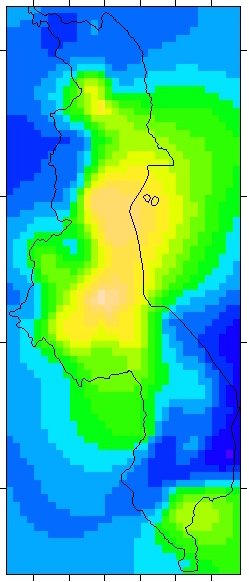
\includegraphics[width=0.265\textwidth]{Figures/Mwisf.png}}}$
\end{frame}

%------------------------------------------------

\begin{frame}
\frametitle{Fernerkundung}
\vspace{0.2cm}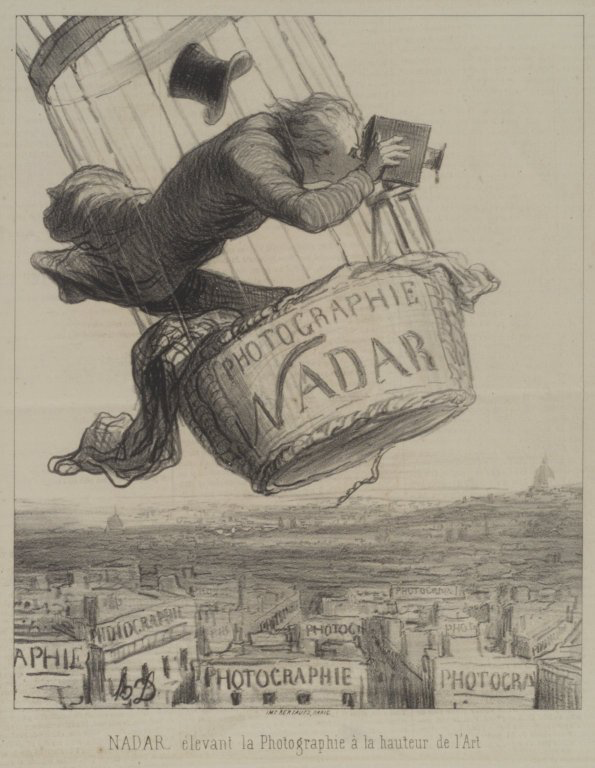
\includegraphics[width=0.3\textwidth]{Figures/remote_sensing.png}
\hspace{1cm}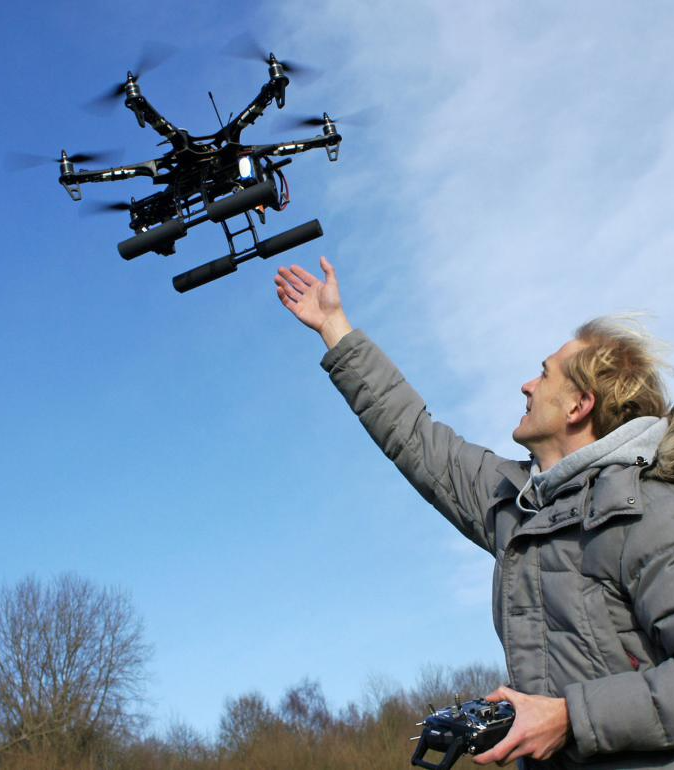
\includegraphics[width=0.34\textwidth]{Figures/drone.png}\\
\tiny Foto: Nadar von Honoré Daumier 
\hspace{1.1cm} Foto: Eine Drone bei der Universität Stockholm\\[0.5cm]
Satelliten, RADAR, LiDAR

\end{frame}

%-----------------------------------------------

\begin{frame}
\frametitle{Fernerkundung \hspace{1cm} \tiny Padmanaban, Bhowmik, Cabral and Wang, 2017. Entropy}
Random Forest Bildklassifizierung
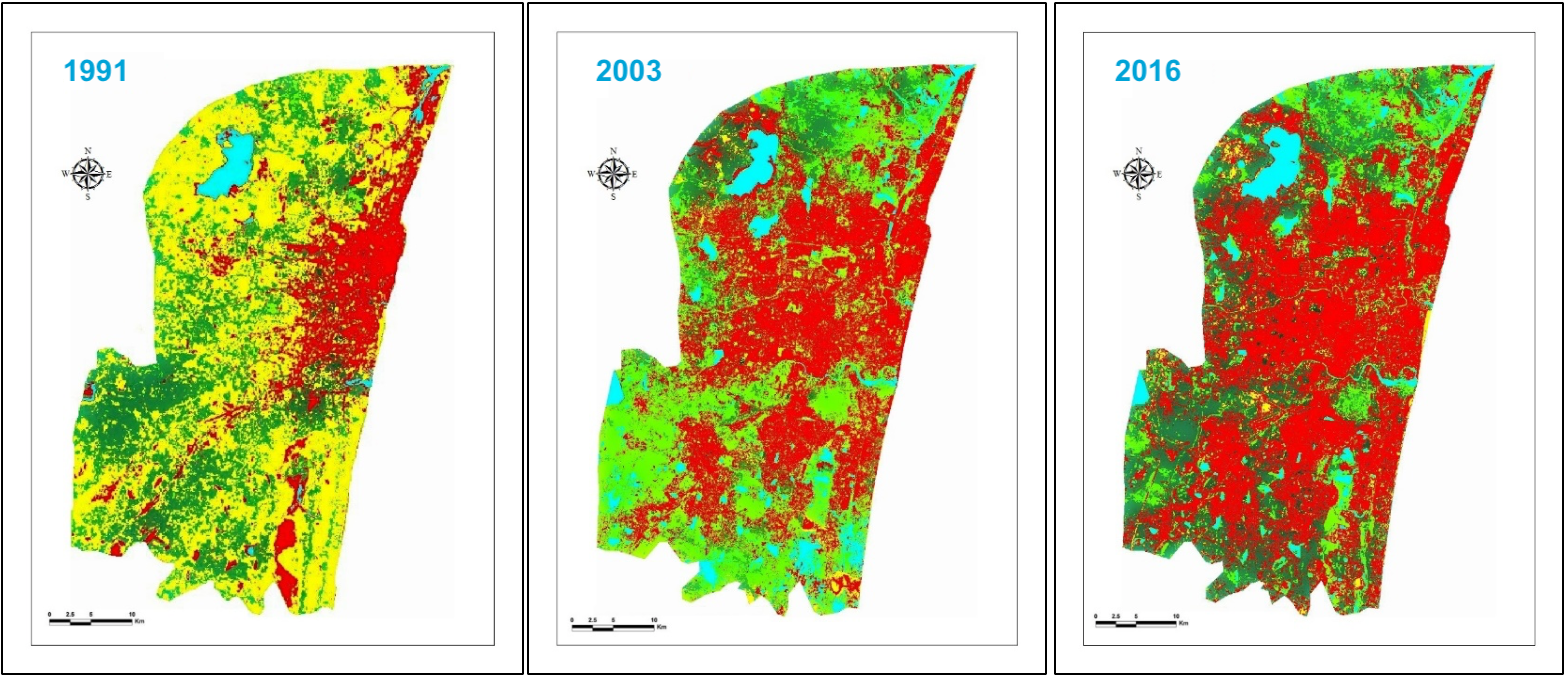
\includegraphics[width=1.05\textwidth]{Figures/RS1.png}\\
Urbanisierung in Chennai
\end{frame}

%-----------------------------------------------

\begin{frame}
\frametitle{Fernerkundung \hspace{1cm} \tiny Padmanaban, Bhowmik, Cabral and Wang, 2017. Entropy}
\onslide<1->
Modell der Landveränderung\\[0.2cm]
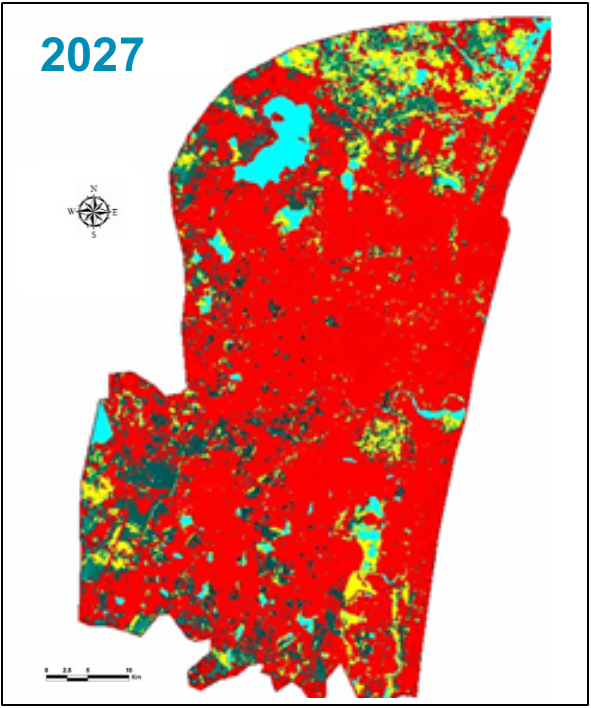
\includegraphics[width=0.44\textwidth]{Figures/RS2.png}
\onslide<2->
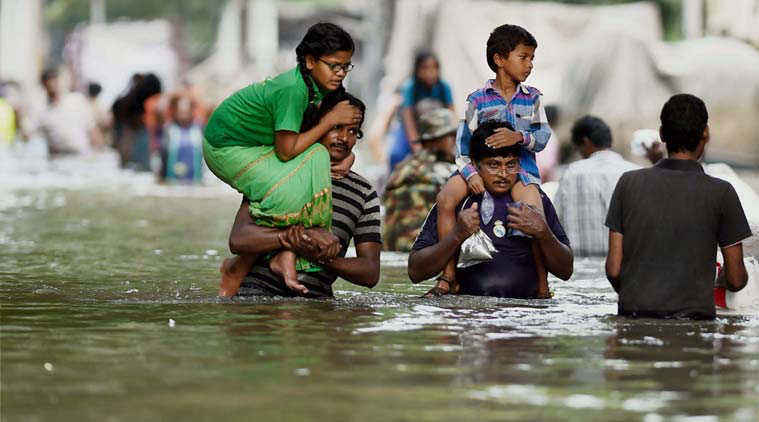
\includegraphics[width=0.53\textwidth]{Figures/chennai.png}\\
\raggedleft\small Verheerende Flut in Chennai, 2018
\end{frame}

%----------------------------------------------

\begin{frame}
\frametitle{}
\centering
\large Anwendung auf den Schutz der Artenvielfalt\\[0.2cm]
\pause
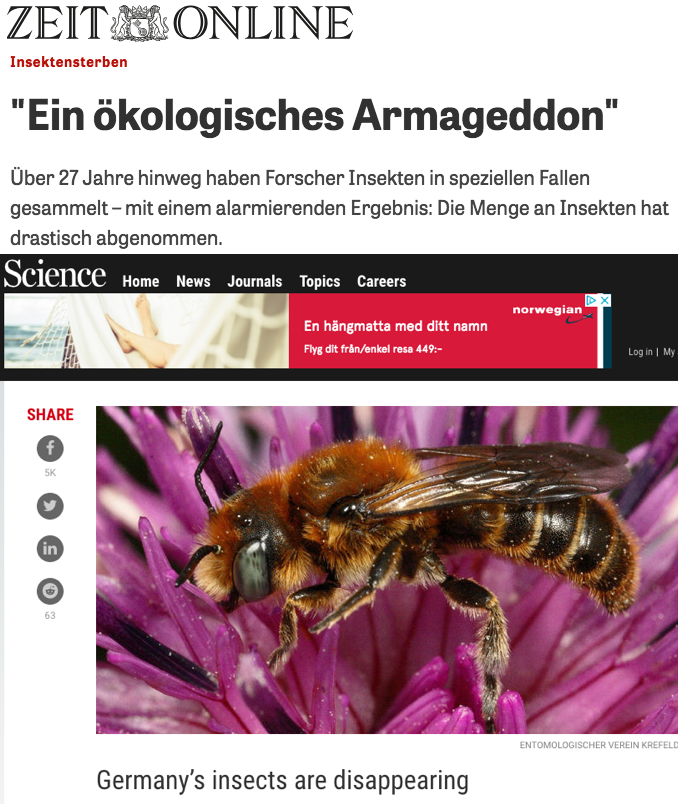
\includegraphics[width=0.5\textwidth]{Figures/news.png}\\
\pause
\small \alert{Klimaauswirkungen auf aquatische Insekten in Deutschland}\\
\scriptsize Bhowmik und Schäfer, 2015. PLOS ONE. e0130025
\end{frame}

%-----------------------------------------------

\begin{frame}[fragile]
  \frametitle{Insekten mit welchen Merkmalen verändern ihre Verteilungsmuster unter dem Klimawandel am stärksten?}
  $\vcenter{\hbox{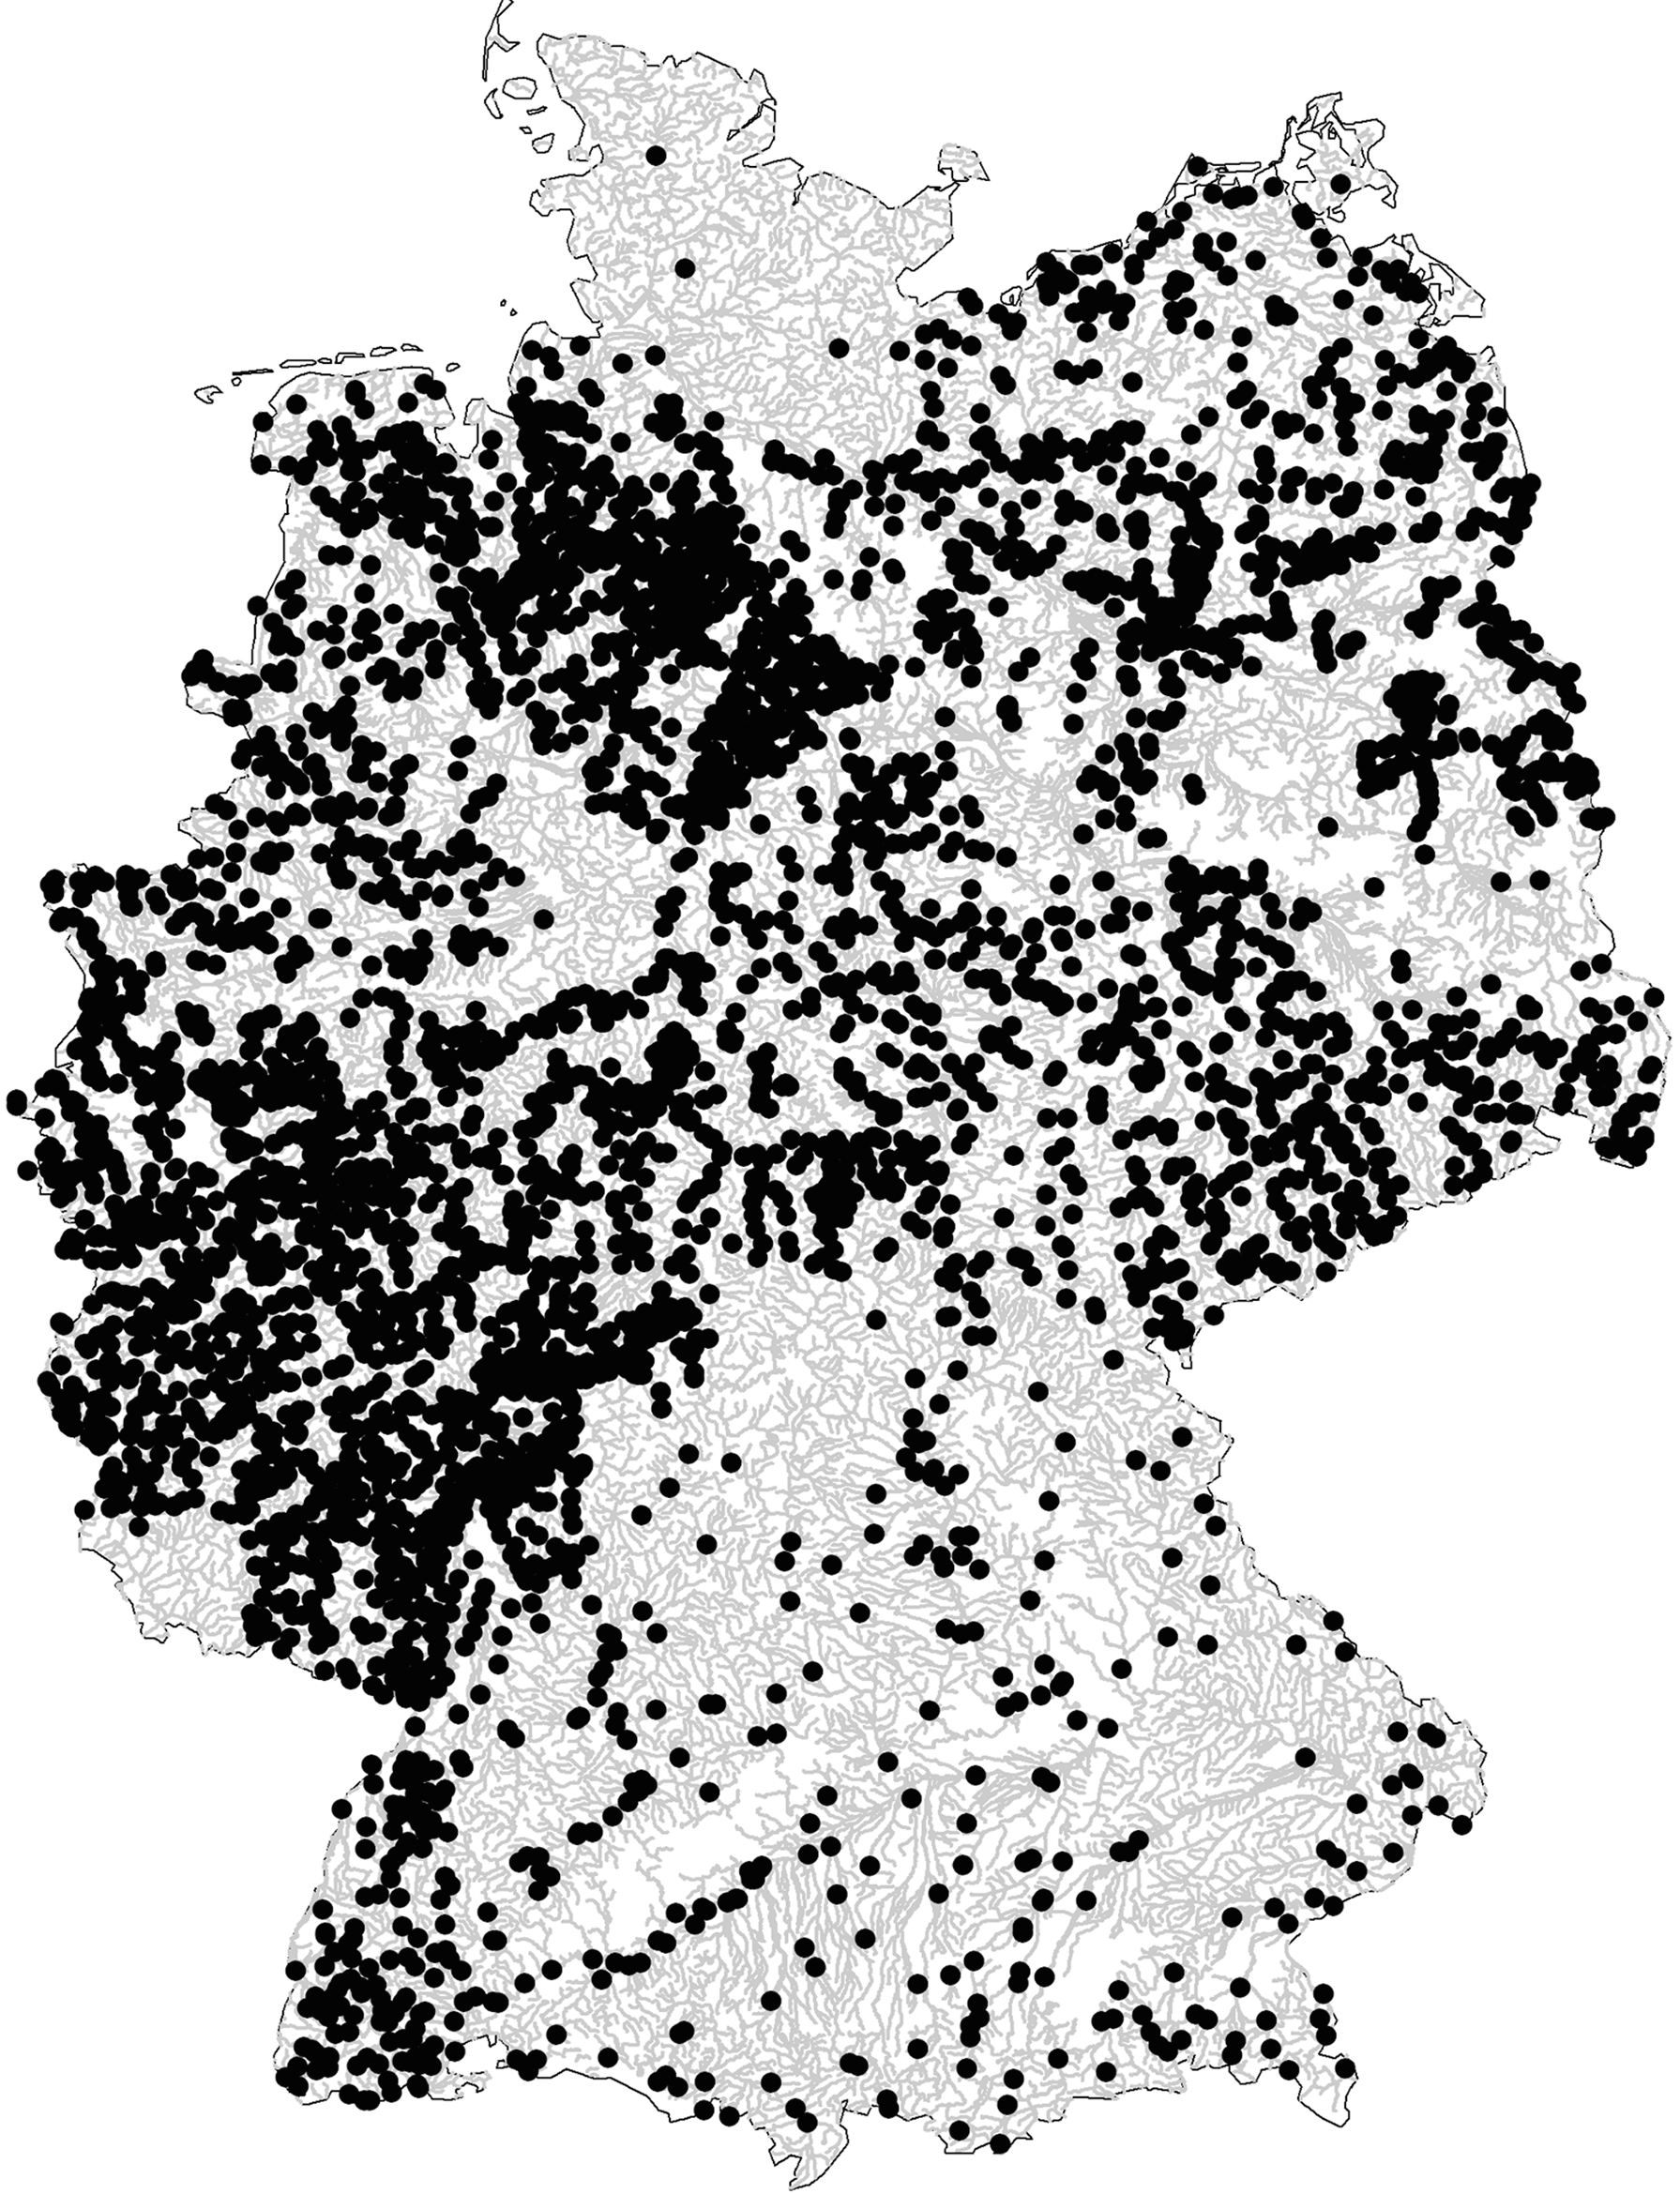
\includegraphics[width=0.40\textwidth]{Figures/Germany_Sites.png}}}$
  \hspace{0.2cm}
  $\vcenter{\hbox{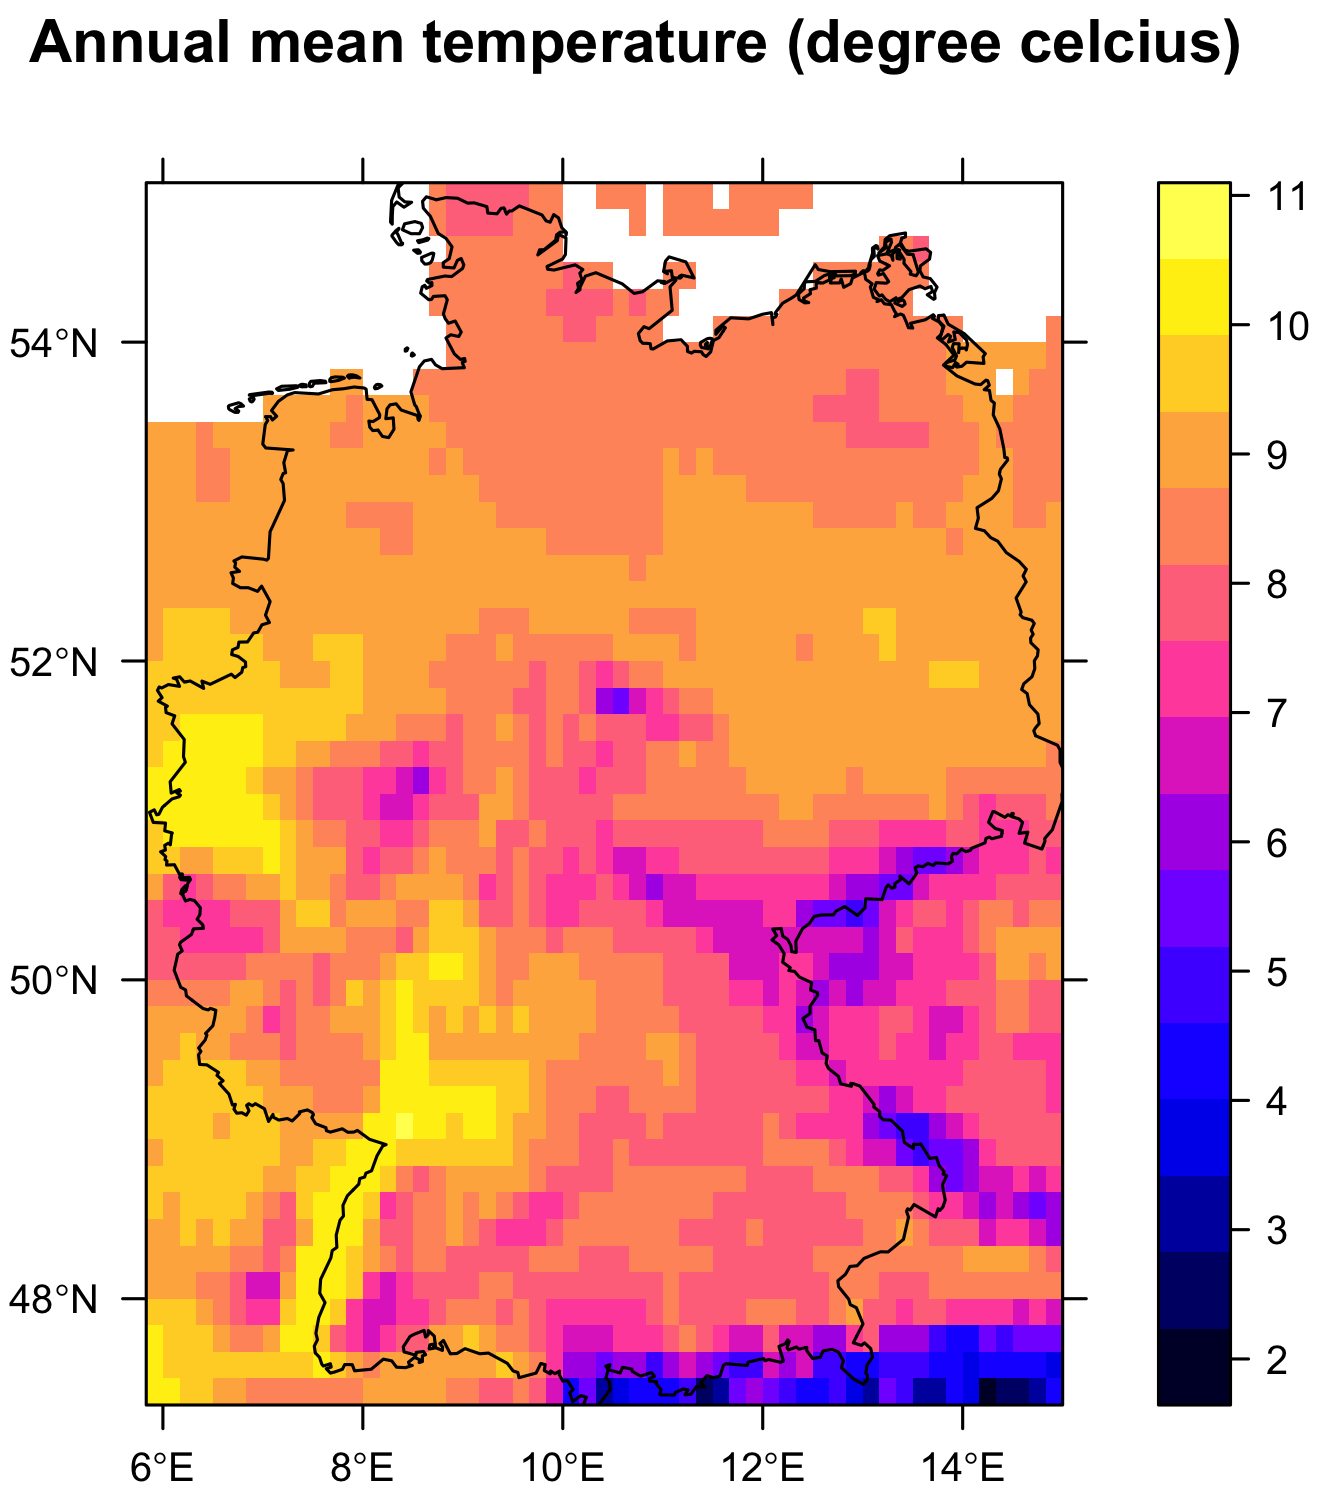
\includegraphics[width=0.45\textwidth]{Figures/Bioclim.png}}}$ \\
  \hspace{5cm} \tiny (Kriticos et al. 2012. Met. Eco. Evo.)\\
  \hspace{-0.5cm}\scriptsize Biomonitoring Daten von 4,752 Fließgewässermesspunkten \& 35 bioklimatischen Variablen 


\end{frame}

%-----------------------------------------------

\begin{frame}[fragile]
  \frametitle{59\% der räumlichen Autokorrelation in abundanz- gewichteten Merkmalen war mit bioklimatischen Indizes assoziiert}
  Anteile an der höchsten räumlichen Autokorrelation:
  \begin{itemize}
  \item in \alert{Temperaturpräferenz (81\%)}, vor allem bei Insekten mit \alert{Kalttemperaturpräferenz (91\%)}
  %\pause
  %e.g. \alert{low dispersal capacity, large body size (>4 cm), low reproductive capacity (semivoltine) and resistance to drought (egg diapause) together explained 55 \% of cold temperature preference}
  \end{itemize}
  \vspace{0.3cm}
  \hspace{1.5cm}
  $\vcenter{\hbox{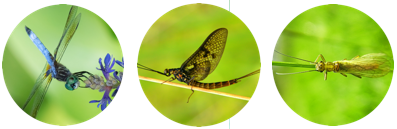
\includegraphics[width=0.7\textwidth]{Figures/Temperature.png}}}$
\end{frame}

%-----------------------------------------------

\begin{frame}
  \frametitle{}
  \centering
  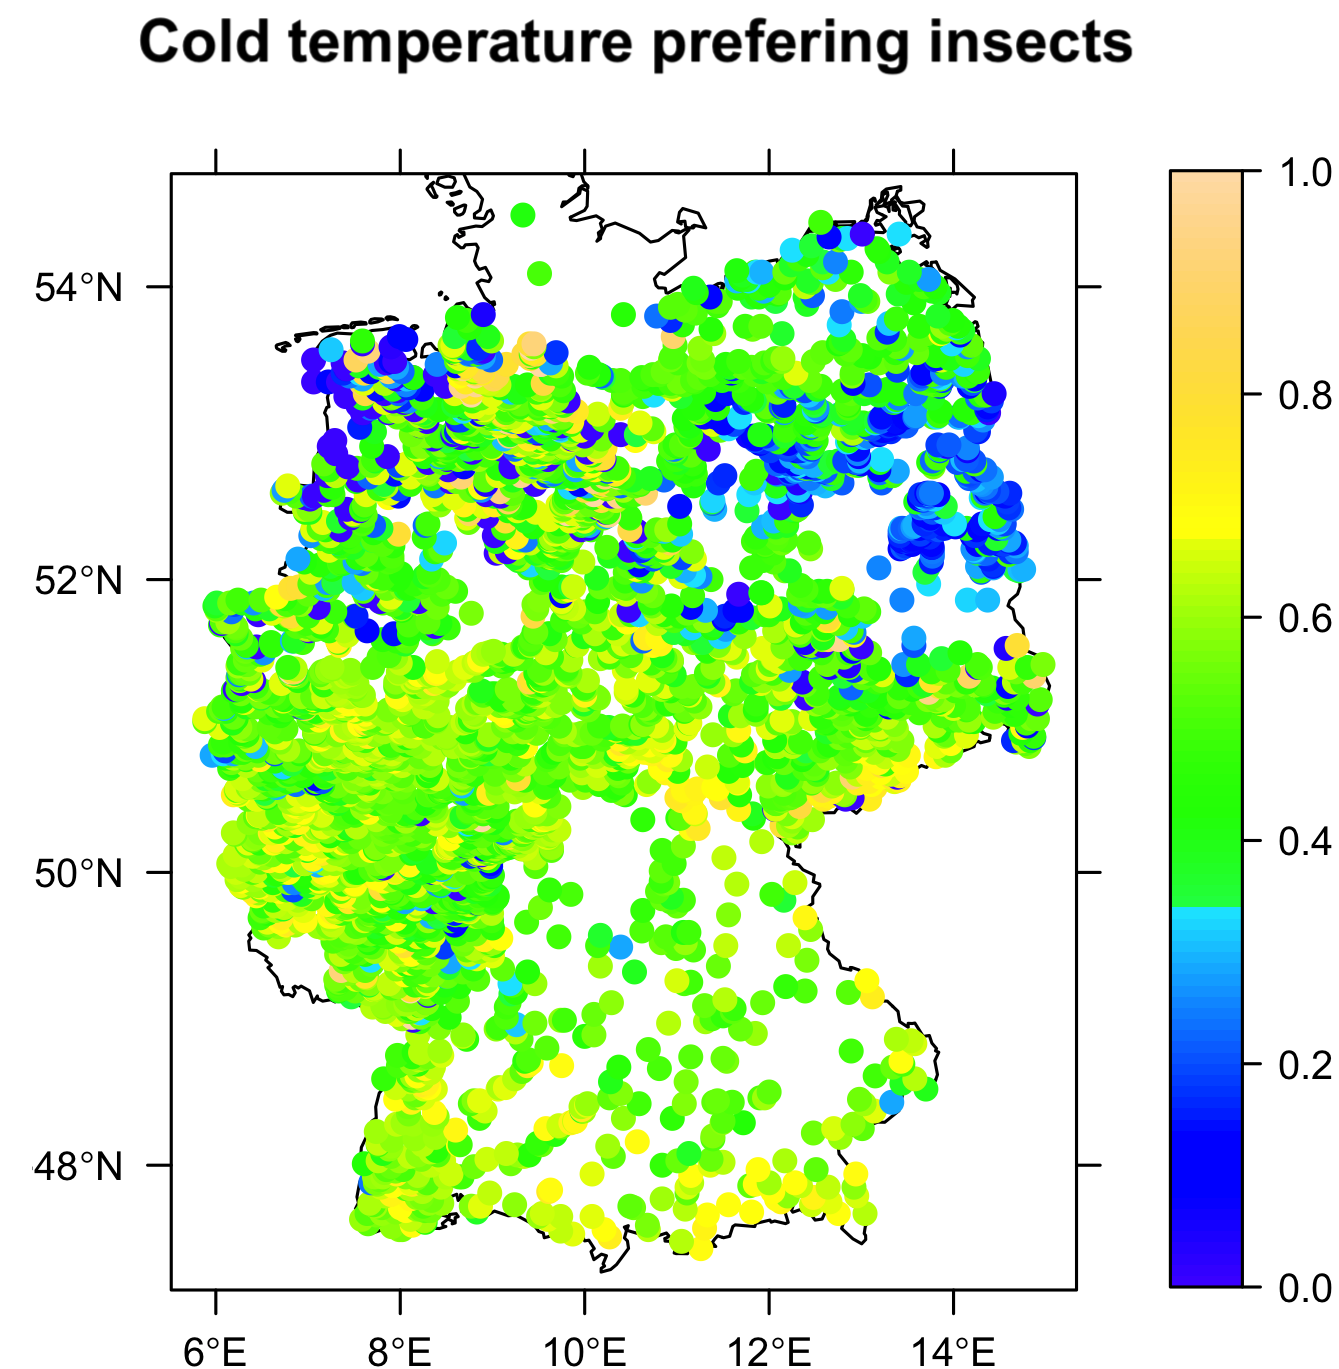
\includegraphics[width=0.515\textwidth]{Figures/Cold.png}
  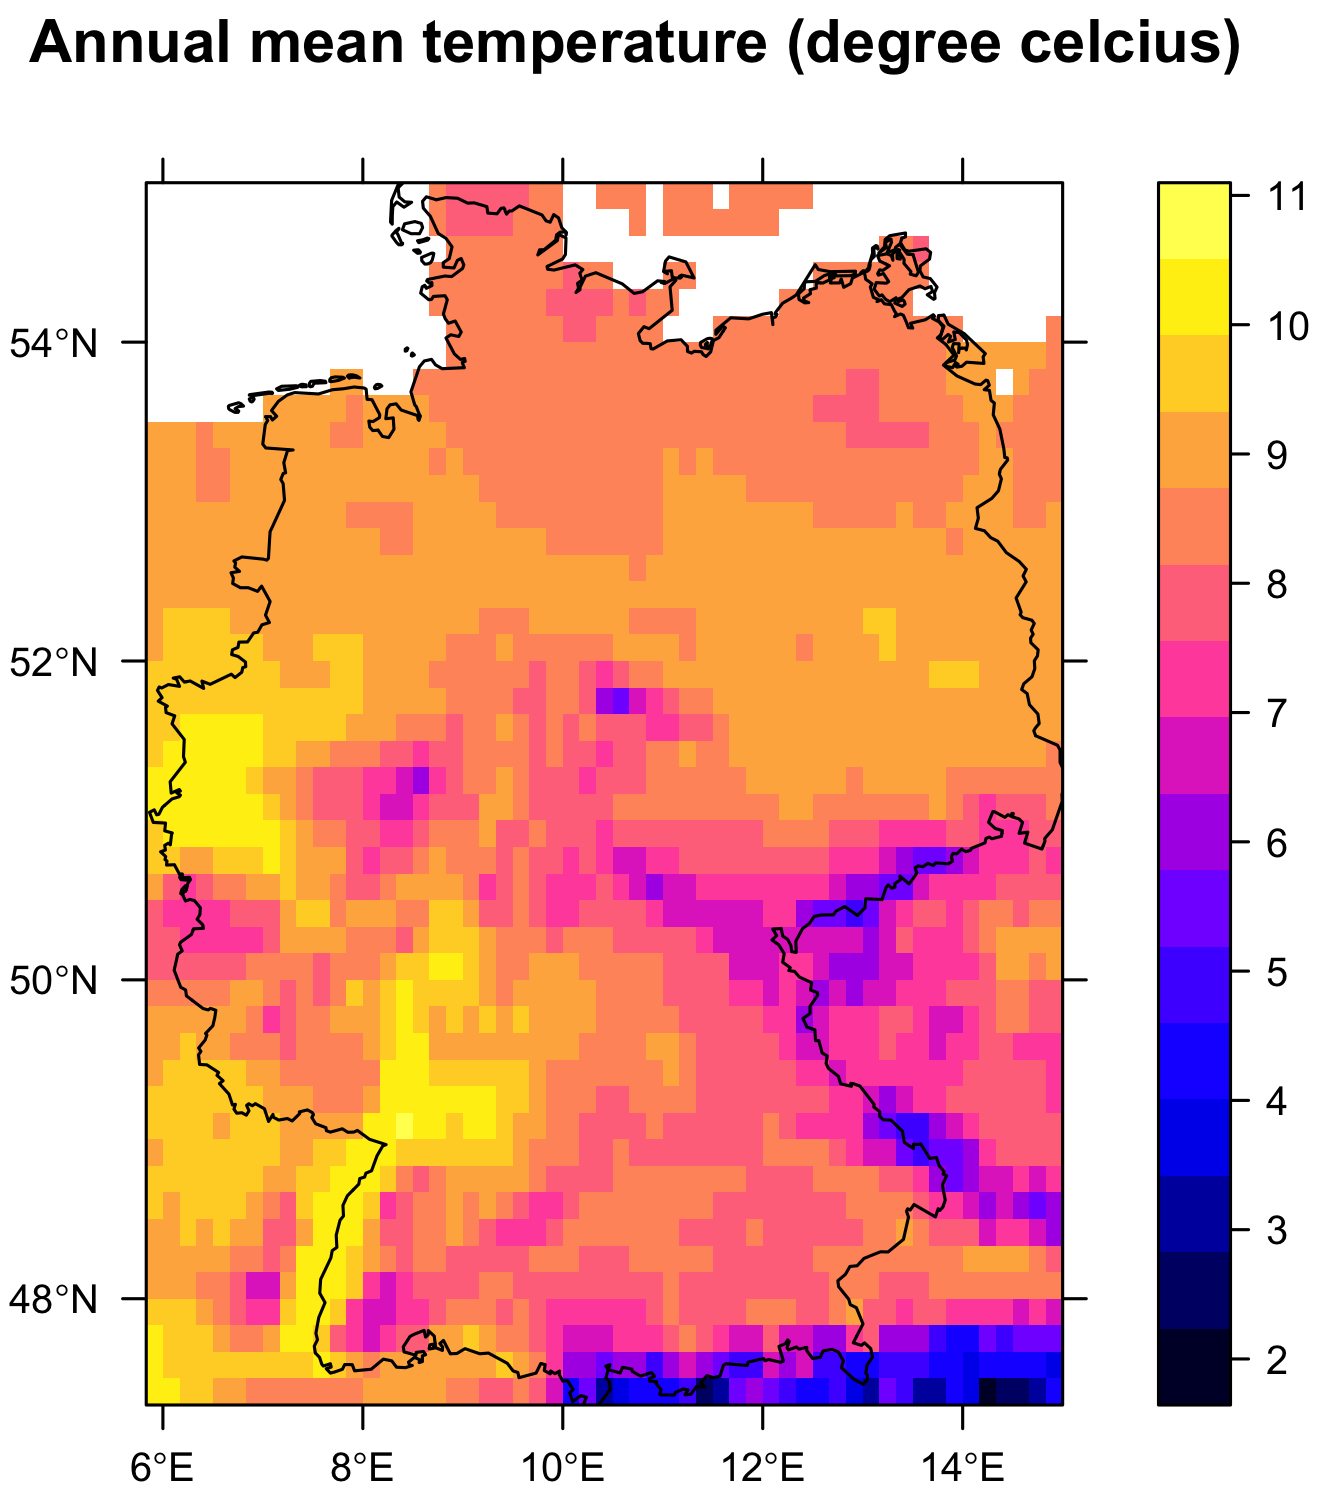
\includegraphics[width=0.465\textwidth]{Figures/Bioclim.png}
\end{frame}

%-----------------------------------------------

\begin{frame}
  \frametitle {Merkmalsbasierte räumliche Metrik für den Schutz der Artenvielfalt}
 \begin{itemize}
  \item \alert{Winter- und Sommertemperatur wird sich im Süden veraussichtlich erhöhen} \footnotesize{(Stocker et al. 2013. IPCC report)}\normalsize
  \pause
  \item\alert{Insekten mit Kalttemperaturpräferenz} (vor allem große Insekten \footnotesize{(Harrison et al. 2010. Bio Sci)}) \normalsize kommen hauptsächlich im Süden vor und \normalsize \alert{werden veraussichtlich in ihrer Verteilung züruckgehen}
  \end{itemize}
  \end{frame}

%-----------------------------------------------

\begin{frame}
\frametitle{}
\centering
\LARGE Vielen Dank für Eure Aufmerksamkeit!\\
\normalsize
\begin{columns}
\begin{column}{0.6\textwidth}
\alert{\textbf{Aufgabe}}\\
Lest die folgenen Buchkapitel aufmerksam durch: \alert{https://github.com/AvitBhowmik/testGU}, und überlegt, welche GIS-Methoden sich für die Planung von Weinbauflächen besonders eignen\\[1cm]
\footnotesize
   Email: \href{mailto:avit.bhowmik@futureearth.org}{\alert{avit.bhowmik@futureearth.org}}\\
   Website: \href{http://avitbhowmik.ml/}{\alert{http://avitbhowmik.ml/}}\\
twitter: \href{https://twitter.com/avitbhowmik}{\alert{@avitbhowmik}}\\
   Google Scholar: \href{https://scholar.google.se/citations?user=laRo5pgAAAAJ&hl=en}{\alert{Dr. Avit K. Bhowmik}}
\end{column}
\begin{column}{0.4\textwidth}
    \begin{center}
     
\includegraphics[width=0.7\textwidth]{Figures/Ques.png}
     \end{center}
\end{column}
\end{columns}
\end{frame}

%------------------------------------------------

\end{document} 